\documentclass[12pt]{article}

\usepackage[margin=1in]{geometry}
\usepackage{amsfonts,amsmath,amssymb}
\usepackage{multicol}

\usepackage{graphicx}
\usepackage{float}
\usepackage[nottoc, notlot, notlof]{tocbibind}
\usepackage{hyperref}
\usepackage{enumitem}
\usepackage{caption}
\usepackage{subcaption}
\usepackage[T1]{fontenc}
\usepackage[utf8]{inputenc}
\usepackage{xcolor}
\newcommand{\leavealine}
{\vskip 0.5cm}


\begin{document}
	{\fontfamily{ppl}\selectfont 
		\begin{center}
			\Large{\textbf{Magnetic Mirror Effect in Magnetron Plasma:}} \\
			\Large{\textbf{Modeling of Plasma Parameters}} \\
		\end{center}
		%\color{blue}

\section{Kinetic Theory of Plasma Physics}
\subsection{The Density Function}
	The kinetic theory describes the plasma as collection of particles whose state (position and velocity) is treated as a random variable with a density function $ f(x, y, z, v_{x}, v_{y}, v_{z}, t) $ which describes the number of particles at position $ (x, y, z) $ at time $ t $ with velocities between $ v_{x} $ and $ v_{x} + dv_{x} $, $ v_{y} $ and $ v_{y} + dv_{y} $, $ v_{z} $ and $ v_{z} + dv_{z} $ in directions $x$, $y$ and $z$ respectively. For a simpler notation $ f(x, y, z, v_{x}, v_{y}, v_{z}, t) $ is denoted as $ f(\textbf{r}, \textbf{v}, t) $.
	The expression $$\displaystyle \int_{all \hspace{0.2cm} v_{x}^{}} dv_{x} \int_{all \hspace{0.2cm} v_{y}^{}} dv_{y} \int_{all \hspace{0.2cm} v_{z}^{}} dv_{z} f(\textbf{r}, \textbf{v}, t) $$ gives the number of particles at position $\textbf{r}$, at time $t$.  For a simple choice of notation, it if often written as $$\displaystyle \int_{all \hspace{0.2cm} \textbf{v}^{}} d^{3}v f(\textbf{r}, \textbf{v}, t) \hspace{0.5cm}\textrm{or} \hspace{0.5cm}\int_{all \hspace{0.2cm} \textbf{v}^{}} d\textbf{v} f(\textbf{r}, \textbf{v}, t)$$ A density function is said to be normalized if $$\displaystyle \int_{all \hspace{0.2cm} \textbf{v}^{}} d\textbf{v} f(\textbf{r}, \textbf{v}, t) = 1$$ Such a density function is also denoted with a hat as $ \hat{f}(\textbf{r}, \textbf{v}, t) $.\\
	\noindent The average velocity $\bar{v}$ for a density function $ \hat{f}(\textbf{r}, \textbf{v}, t) $ is calculated as  $$\displaystyle \int_{all \hspace{0.2cm} \textbf{v}^{}} d\textbf{v} \hspace{0.2cm} v f(\textbf{r}, \textbf{v}, t)$$ Various other features of the distribution are: the Root Mean Square velocity $v_{rms}$, the average absolute velocity $|\bar{v}|$, the average velocity in $z$ direction $\bar{v_{z}}$, etc.\\
	
	\noindent One important density function often used in the kinetic theory of plasma is the Maxwell-Boltzmann distribution often called the Maxwellian which has the density function 
	\begin{equation}
		\label{eqn:maxwellian}
		\widehat{f_{M}} := \hat{f}(\textbf{r}, \textbf{v}, t) = \left(\frac{m}{2\pi KT}\right)^{\frac{3}{2}} \mathrm{exp}\left(-\frac{v^{2}}{v_{th}^{2}}\right)
	\end{equation} where $$v_{th}^{2} = \frac{2 K T}{m}$$ Some features of the Maxwellian are:
	$$ v_{rms} = \sqrt{\frac{3 K T}{m}} \mathrm{,} |\bar{v}| = 2\sqrt{\frac{2 K T}{\pi m}} \mathrm{,} |\bar{v_{z}}| = \sqrt{\frac{2 K T}{\pi m}} \mathrm{,} \bar{v_{z}} = 0 $$
	
\subsection{Equation of Motion}
	The dynamics of the system is described by change in the density function. In a one dimensional consideration, in a frame moving with each particle, this is described as $$ \frac{df}{dt} = \frac{\partial f}{\partial t} + \frac{\partial f}{\partial x} \frac{d x}{d t} + \frac{\partial f}{\partial v_{x}} \frac{d v_{x}}{d t}$$ as $ f $ is a function of the position $x$, the velocity $v_{x}$ and time $t$ in general. This is also written as 
	$$ \frac{df}{dt} = \frac{\partial f}{\partial t} + \frac{\partial f}{\partial x} v_{x} + \frac{\partial f}{\partial v_{x}} a_{x} $$ replacing the expressions for velocity and acceleration. If there were no external disturbance to the system, the equation of motion would be
	$$ \frac{\partial f}{\partial t} + \frac{\partial f}{\partial x} v_{x} + \frac{\partial f}{\partial v_{x}} a_{x} = 0$$ or simply 
	\begin{equation}
		\label{eqn:eom}
		\frac{df}{dt} = 0
	\end{equation} 
	
	\noindent In three dimensions it is easy to see that
	$$ \frac{df}{dt} = \frac{\partial f}{\partial t} + \frac{\partial f}{\partial x} \frac{d x}{d t} + \frac{\partial f}{\partial v_{x}} \frac{d v_{x}}{d t} + \frac{\partial f}{\partial y} \frac{d y}{d t} + \frac{\partial f}{\partial v_{y}} \frac{d v_{y}}{d t} + \frac{\partial f}{\partial z} \frac{d z}{d t} + \frac{\partial f}{\partial v_{z}} \frac{d v_{z}}{d t}$$ as $ f $ is a function of the position $(x,y,z)$, the velocity $(v_{x},v_{y},v_{z})$ and time $t$ in general. Substituting the expressions for velocity and acceleration, it is also written as $$ \frac{df}{dt} = \frac{\partial f}{\partial t} + \frac{\partial f}{\partial x} v_{x} + \frac{\partial f}{\partial v_{x}} a_{x} + \frac{\partial f}{\partial y} v_{y} + \frac{\partial f}{\partial v_{y}} a_{y} + \frac{\partial f}{\partial z} v_{z} + \frac{\partial f}{\partial v_{z}} a_{z}$$ which is often written as $$\frac{df}{dt} = \frac{\partial f}{\partial t} + \textbf{v} \cdot \nabla f + \textbf{a} \cdot {\partial}_{\textbf{v}} f $$  hence the equation of motion for the case with no external disturbance would be $$\frac{\partial f}{\partial t} + \textbf{v} \cdot \nabla f + \textbf{a} \cdot {\partial}_{\textbf{v}} f = 0$$ which is again the simple expression in equation (\ref{eqn:eom}). \\
	
	\noindent A special case of this is when the force acting on the particles in the Lorentz force. In such a case this equation is written as
	\begin{equation}
		\label{eqn:vlasov}
		\frac{\partial f}{\partial t} + \textbf{v} \cdot \nabla f + \frac{q}{m} \left(\mathrm{\textbf{E}}+\textbf{v} \times \mathrm{\textbf{B}} \right) \cdot {\partial}_{\textbf{v}} f = 0
	\end{equation} and is called the Vlasov equation.
	
	\noindent Including the external disturbances caused due to Electric and Magnetic Fields or any other force would have a non zero term on the right hand side of the equation (\ref{eqn:eom}). The equation 
	\begin{equation}
		\label{eqn:boltzmann}
		\frac{df}{dt} = \left(\frac{\partial f}{\partial t}\right)_{c} 
	\end{equation} where the term on the right hand side describes the change of the density function due to collisions between particles is called the Boltzmann equation which is often written as $$\frac{\partial f}{\partial t} + \textbf{v} \cdot \nabla f + \frac{\textbf{F}}{m} \cdot {\partial}_{\textbf{v}} f = \left(\frac{\partial f}{\partial t}\right)_{c}$$The collision term is often used to describe electromagnetic Coulomb between two particles, collisions with uncharged particles, etc.
	

\section{Magnetic Mirror}
	The magnetic mirror effect can first be illustrated with a 	single particle. For the simple case, it is assumed that there is no electric field acting on the particle, the magnetic field is cylindrically symmetric and the gradient of the magnetic field is only along the axial direction of the cylinder, the $z$ direction.  The magnetic moment $$\mu = \frac{m v_{\perp}^{2}}{2B_{z}} $$ of the particle is an adiabatic invariant of the particle motion and hence is approximately conserved for a magnetic field whose $z$ component $B_{z}$ does not vary too much . The kinetic energy$$ KE = \frac{1}{2}m v^{2}$$ of the particle is also approximately conserved. Writing $v_{\perp} = v sin \theta$,
	$$\frac{\mu}{KE} = \frac{sin^{2}\theta}{B_{z}}$$ is also a conserved quantity. This means that as $B$ increases (within a small range), $sin^{2}\theta$ increases as well and so does $|sin\theta|$ which means that $|v_{\perp}|$ increases and since $v$ is conserved, $v_{\parallel}$ decreases to zero. When $v_{\parallel} = 0$, the particle is no longer moving in the $z$ direction, but is moving with velocity $v$ in the plane perpendicular to $z$ direction. The $v_{\parallel}$ then increases in the opposite direction as the particle moves towards decreasing $B$ because of the Lorentz force. Such a particle is seen as being reflected due to the configuration of the magnetic field and hence such a configuration of the magnetic field is called a magnetic mirror. Particles whose $v_{\parallel}$ does not decrease to 0 while the value of $B$ is decreasing, escape from the magnetic mirror configuration. \\
	
	\noindent This can be written as
	$$ \frac{sin^{2}\theta}{B_{z}} =  \frac{sin^{2}\theta_{0}}{B_{z_{0}}} $$ \\
	
	\color{blue}
	\textbf{TO DO 1} \\
	\color{red} 
	\textbf{I am still a bit confused on how to use this for a dynamic velocity distribution to get an expression for reflected and lost flux. So things after here in this section are not entirely clear.}
	\color{black}\\
	
	if the velocity of the particle (and hence $sin\theta$) and the magnetic field in the $z$ direction $B_{z}$ are known at some location to be $sin\theta_{0}$ and $B_{z_{0}}$ respectively.
	The particle that either just escapes the magnetic mirror or is just reflected would have $ v_{\perp} = v $ and $ sin\theta = 1 $ $$ sin^{2}\theta = \frac{B_{z}}{B_{z_{0}}} \hspace{0.2cm} sin^{2}\theta_{0}$$
	Since $$ sin^{2}\theta \leq 1 \hspace{2cm} \frac{B_{z}}{B_{z_{0}}} \hspace{0.2cm} sin^{2}\theta_{0} \leq 1$$\\
	
	\noindent The reflected fraction is given by 
	$$ f_{loss} = \frac{\displaystyle \int_{loss \hspace{0.1cm} cone}^{} f(\textbf{r}, \textbf{v}, t)  \hspace{0.2 cm} d \textbf{v}}{\displaystyle \int_{all \hspace{0.2 cm}\textbf{v}}^{} f(\textbf{r}, \textbf{v}, t) \hspace{0.2 cm} d \textbf{v}} = \frac{\int_{0}^{2 \pi} d \phi \left[ \int_{0}^{\theta_{0}} sin \theta d \theta + \int_{\pi - \theta_{0}}^{\pi} sin \theta d \theta \right] \int_{all v}^{} \frac{\displaystyle  f(\textbf{r}, \textbf{v}, t)  \hspace{0.2 cm} dv}{4 \pi v^{2}}}{\int_{0}^{2 \pi} d \phi \int_{0}^{\pi} sin \theta d \theta \int_{all v}^{} \frac{\displaystyle  f(\textbf{r}, \textbf{v}, t)  \hspace{0.2 cm} dv}{4 \pi v^{2}}} = 1 - cos\theta_{0}$$
	
\section{Parabolic Density Functions}
	The simplest density function to try would be to have all particles have the same velocity i.e. a Dirac delta function distribution. Another simple distribution would be a uniform distribution between two velocities, where a particle is equally likely to have any velocity in the range.
	
	\subsection{Definitions}
	The uniform distribution describes a collection of particles where a particle chosen at random is equally likely to have any velocity in the range.
	\[ f_{0} = 
	\begin{cases} 
		\frac{1}{2 v_{a}} & -v_{a}\leq v\leq v_{a} \\
		0 & else 
	\end{cases}
	\] \\ which is already normalized. The Dirac delta-like distribution would describe all the particles having the same velocity.
	\[ f_{\delta} = 
	\begin{cases} 
		1 & v = v_{a} \\
		0 & else 
	\end{cases}
	\]
	\begin{figure}[H]
		\begin{multicols}{2}
			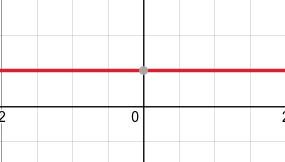
\includegraphics[width=\linewidth, height=5cm]{uniform.png} \caption{$f_{0}$} \par
			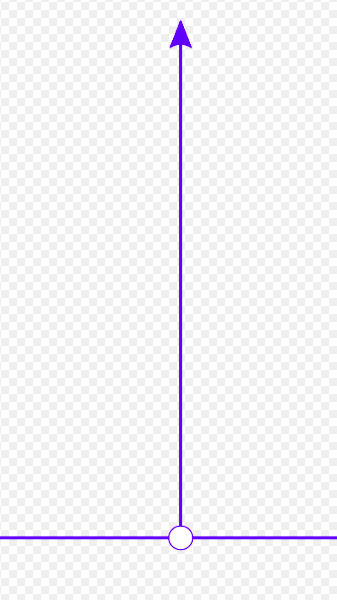
\includegraphics[width=\linewidth, height=5cm]{dirac.png} \caption{$f_{\delta}$} \par
		\end{multicols}
	\end{figure}
	The figure for $f_{0}$ was generated using desmos graphing calculator while the figure for $f_{\delta}$ was snipped from the image in wikipedia for the Dirac delta function. \\
	
	\noindent However, uniform and delta distributions are not very realistic in a system of large number of particles. Parabolic functions in a given range also seem like interesting distributions and yet simple to work with. After some trial and error, two functions that seem interesting are:
	\[ f_{1} = 
	\begin{cases} 
		1- \frac{v^{2}}{2 v_{a}^2} & -v_{a}\leq v\leq v_{a} \\
		0 & else 
	\end{cases}
	\]
	\[ f_{2} = 
	\begin{cases}
		1 + \frac{v^{2}}{2 v_{a}^2} & v_{a}\leq v\leq v_{a} \\
		0 & else
	\end{cases}\]  
	
	These functions can be normalized as
	$$ \int_{v_{x} = -v_{a}}^{v_{x} = v_{a}} dv_{x} \int_{v_{y} = -v_{a}}^{v_{y} = v_{a}} dv_{y} \int_{v_{z} = -v_{a}}^{v_{z} = v_{a}} dv_{z} \hspace{0.2cm}c_{0}  \left(1 - \frac{v_{x}^{2}+v_{y}^{2}+v_{z}^{2}}{2 v_{a}^2}\right) = 1 \hspace{2cm} \mathrm{and}$$
	$$ \int_{v_{x} = -v_{a}}^{v_{x} = v_{a}} dv_{x} \int_{v_{y} = -v_{a}}^{v_{y} = v_{a}} dv_{y} \int_{v_{z} = -v_{a}}^{v_{z} = v_{a}} dv_{z} \hspace{0.2cm} c_{0}  \left(1 + \frac{v_{x}^{2}+v_{y}^{2}+v_{z}^{2}}{2 v_{a}^2}\right) = 1 \hspace{2cm} \mathrm{giving}$$
	
	\[ \hat{f_{1}} = 
	\begin{cases} 
		\frac{1}{4 v_{a}^{3}} \left(1 - \frac{v^{2}}{2 v_{a}^2}\right) & -v_{a}\leq v\leq v_{a} \\
		0 & else 
	\end{cases}
	\]
	\[ \hat{f_{2}} = 
	\begin{cases}
		\frac{1}{12 v_{a}^{3}} \left(1 + \frac{v^{2}}{2 v_{a}^2}\right) & v_{a}\leq v\leq v_{a} \\
		0 & else
	\end{cases}\] 
	
	\noindent The graph of these functions (considering $v$ as a single variable) were generated using desmos graphing calculator. The figures represent $\hat{f_{1}}$ and $\hat{f_{2}}$ extrapolated to beyond the defined range.
	\begin{figure}[H]
		\begin{multicols}{2}
			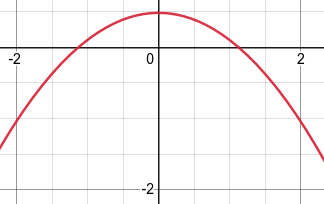
\includegraphics[width=\linewidth, height=5cm]{first.png} \caption{$\hat{f_{1}}$} \par
			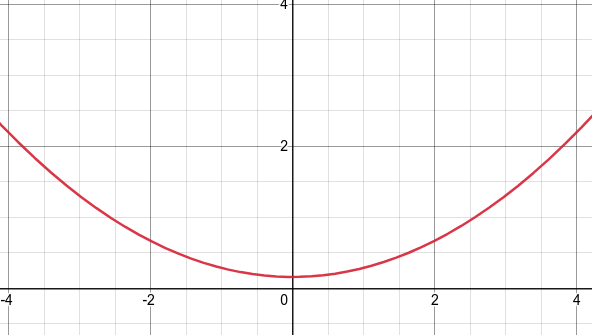
\includegraphics[width=\linewidth, height=5cm]{second.png} \caption{$\hat{f_{2}}$} \par
		\end{multicols}
	\end{figure}

	\noindent In the upper half of the plane, $\hat{f_{1}}$ looks approximately like a Gaussian distribution which the Maxwellian is for a distribution of velocity (not speed) for a fixed temperature. $\hat{f_{2}}$ is sort of the opposite of $\hat{f_{1}}$. But given that the functions are defined in a limited range, the integrals do not diverge.
	
	\subsection{Plugging into the Vlasov equation}
	One good exercise is to check what happens when plugging in  $\hat{f_{1}}$ , $\hat{f_{2}}$ and $f_{M}$ in  the collisionless Vlasov equation
	$$ \frac{\partial f}{\partial t} + \textbf{v} \cdot \nabla f + \frac{q}{m} \left(\mathrm{\textbf{E}}+\textbf{v} \times \mathrm{\textbf{B}} \right) \cdot {\partial}_{\textbf{v}} f = 0 $$
	For all three of the density functions
	$$\frac{\displaystyle \partial f}{\displaystyle \partial t} = 0 \mathrm{,} \hspace{1cm} \frac{\displaystyle \partial f}{\displaystyle \partial x} = 0 \mathrm{,} \hspace{1cm} \frac{\displaystyle \partial f}{\displaystyle \partial y} = 0 \mathrm{,} \hspace{1cm} \frac{\displaystyle \partial f}{\displaystyle \partial z} = 0 $$ as all three have no explicit dependence on position or time. The Vlasov equation then becomes $$ \left(\mathrm{\textbf{E}}+\textbf{v} \times \mathrm{\textbf{B}} \right) \cdot {\partial}_{\textbf{v}} f = 0 $$ which is 
	$$ \left(E_{x} + v_{y} B_{z} - v_{z} B_{y}\right) \frac{\displaystyle \partial f}{\displaystyle \partial v_{x}} + \left(E_{y} + v_{z} B_{x} - v_{x} B_{z}\right) \frac{\displaystyle \partial f}{\displaystyle \partial v_{y}} + \left(E_{z} + v_{x} B_{y} - v_{y} B_{x}\right) \frac{\displaystyle \partial f}{\displaystyle \partial v_{z}} = 0$$
	For the Maxwellian, $$ 	\widehat{f_{M}} := \hat{f}(\textbf{r}, \textbf{v}, t) = \left(\frac{m}{2\pi KT}\right)^{\frac{3}{2}} \mathrm{exp}\left(-\frac{v^{2}}{v_{th}^{2}}\right) $$
	$$\frac{\displaystyle \partial f_{M}}{\displaystyle \partial v_{x}} = \left(\frac{m}{2 \pi K T}\right)^{\frac{3}{2}}  \mathrm{exp} \left(\frac{-v^{2}}{v_{th}^{2}}\right)\left(\frac{-2 v_{x}}{v_{th}^{2}}\right)\mathrm{,} \hspace{1cm} \frac{\displaystyle \partial f_{M}}{\displaystyle \partial v_{y}} = \left(\frac{m}{2 \pi K T}\right)^{\frac{3}{2}}  \mathrm{exp} \left(\frac{-v^{2}}{v_{th}^{2}}\right)\left(\frac{-2 v_{y}}{v_{th}^{2}}\right) \mathrm{,}$$ $$\frac{\displaystyle \partial f_{M}}{\displaystyle \partial v_{z}} = \left(\frac{m}{2 \pi K T}\right)^{\frac{3}{2}}  \mathrm{exp} \left(\frac{-v^{2}}{v_{th}^{2}}\right)\left(\frac{-2 v_{z}}{v_{th}^{2}}\right)$$
	plugging in, the equation becomes
	$$\left(\frac{m}{2 \pi K T}\right)^{\frac{3}{2}}  \mathrm{exp} \left(\frac{-v^{2}}{v_{th}^{2}}\right)\left(\frac{-2}{v_{th}^{2}}\right) \left[v_{x}\left( E_{x} + v_{y} B_{z} - v_{z} B_{y} \right) + v_{y} \left( E_{y} + v_{z} B_{x} - v_{x} B_{z} \right) + \right.$$ $$\left. v_{z} \left(E_{z} + v_{x} B_{y} - v_{y} B_{x}\right) \right] = 0$$
	which gives
	$$v_{x} E_{x} + v_{y} E{y} + v_{z} E_{z} = 0$$
	which can also be written as 
	\begin{equation}
		\label{eqn:MaxwellInVlasov}
		\textbf{v} \cdot \mathrm{\textbf{E}} = 0
	\end{equation} 
	which says that the particles move perpendicular to the electric field which is characteristic of the Lorentz force.
	For the parabolic functions,
	\[ \hat{f_{1}} = 
	\begin{cases} 
		\frac{1}{4 v_{a}^{3}} \left(1 - \frac{v^{2}}{2 v_{a}^2}\right) & -v_{a}\leq v\leq v_{a} \\
		0 & else 
	\end{cases}
	\]
	\[ \hat{f_{2}} = 
	\begin{cases}
		\frac{1}{12 v_{a}^{3}} \left(1 + \frac{v^{2}}{2 v_{a}^2}\right) & v_{a}\leq v\leq v_{a} \\
		0 & else
	\end{cases}\] 
	\[ \frac{\displaystyle \partial \hat{f_{1}}}{\displaystyle \partial v_{x}} = 
	\begin{cases} 
		\frac{1}{4 v_{a}^{3}} \left(\frac{- 2 v_{x}}{2 v_{a}^2}\right) & -v_{a} < v < v_{a} \\
		\mathrm{undefined} & v = - v_{a}, v = v_{a} \\
		0 & else 
	\end{cases}
	\]
	\[ \frac{\displaystyle \partial \hat{f_{1}}}{\displaystyle \partial v_{y}} = 
	\begin{cases} 
		\frac{1}{4 v_{a}^{3}} \left(\frac{- 2 v_{y}}{2 v_{a}^2}\right) & -v_{a} < v < v_{a} \\
		\mathrm{undefined} & v = - v_{a}, v = v_{a} \\
		0 & else 
	\end{cases}
	\]
	\[ \frac{\displaystyle \partial \hat{f_{1}}}{\displaystyle \partial v_{z}} = 
	\begin{cases} 
		\frac{1}{4 v_{a}^{3}} \left(\frac{- 2 v_{z}}{2 v_{a}^2}\right) & -v_{a} < v < v_{a} \\
		\mathrm{undefined} & v = - v_{a}, v = v_{a} \\
		0 & else 
	\end{cases}
	\]
	\[ \frac{\displaystyle \partial \hat{f_{2}}}{\displaystyle \partial v_{x}} = 
	\begin{cases} 
		\frac{1}{12 v_{a}^{3}} \left(\frac{2 v_{x}}{2 v_{a}^2}\right) & -v_{a} < v < v_{a} \\
		\mathrm{undefined} & v = - v_{a}, v = v_{a} \\
		0 & else 
	\end{cases}
	\]
	\[ \frac{\displaystyle \partial \hat{f_{2}}}{\displaystyle \partial v_{y}} = 
	\begin{cases} 
		\frac{1}{12 v_{a}^{3}} \left(\frac{2 v_{y}}{2 v_{a}^2}\right) & -v_{a} < v < v_{a} \\
		\mathrm{undefined} & v = - v_{a}, v = v_{a} \\
		0 & else 
	\end{cases}
	\]
	\[ \frac{\displaystyle \partial \hat{f_{2}}}{\displaystyle \partial v_{z}} = 
	\begin{cases} 
		\frac{1}{12 v_{a}^{3}} \left(\frac{2 v_{z}}{2 v_{a}^2}\right) & -v_{a} < v < v_{a} \\
		\mathrm{undefined} & v = - v_{a}, v = v_{a} \\
		0 & else 
	\end{cases}
	\]
	In the range $v \in \mathbb{R} \textbackslash \left[-v_{a}, v_{a}\right] $ the equation becomes $0 = 0$ which is trivial. The equation becomes undefined for $v = v_{a}$ and 
	$v = - v_{a}$ but we can ignore that for now. In the interesting range of $v \in \left(-v_{a}, v_{a}\right) $, the equation becomes 
	$$ \frac{1}{4 v_{a}^{3}} \left(\frac{- 2}{2 v_{a}^2}\right) \left[v_{x}\left( E_{x} + v_{y} B_{z} - v_{z} B_{y} \right) + v_{y} \left( E_{y} + v_{z} B_{x} - v_{x} B_{z} \right) + v_{z} \left(E_{z} + v_{x} B_{y} - v_{y} B_{x}\right) \right] = 0 $$
	for $\hat{f_{1}}$ and
	$$ \frac{1}{12 v_{a}^{3}} \left(\frac{2}{2 v_{a}^2}\right) \left[v_{x}\left( E_{x} + v_{y} B_{z} - v_{z} B_{y} \right) + v_{y} \left( E_{y} + v_{z} B_{x} - v_{x} B_{z} \right) + v_{z} \left(E_{z} + v_{x} B_{y} - v_{y} B_{x}\right) \right] = 0 $$
	for $\hat{f_{2}}$ which both give the same equation as $\widehat{f_{M}}$
	$$v_{x} E_{x} + v_{y} E{y} + v_{z} E_{z} = 0 \hspace{1cm}\mathrm{or}\hspace{1cm}\textbf{v} \cdot \mathrm{\textbf{E}} = 0$$
	\noindent $\hat{f_{1}}$ and $\hat{f_{2}}$ behave similar to $\hat{f_{M}}$ when plugged into the Vlasov equation.
		
	\subsection{Plugging into the expression for Magnetic Mirror}
	\noindent Since the quantity $\frac{\displaystyle sin^{2}\theta}{\displaystyle B_{z}}$ is conserved in a magnetic mirror, it is a good exercise to calculate the average value or expectation of $sin^{2}\theta$, $\left\langle sin^{2}\theta\right\rangle = \left\langle \frac{\displaystyle v_{\perp}^{2}}{\displaystyle v^{2}}\right\rangle = \left\langle \frac{\displaystyle v_{x}^{2} + v_{y}^{2}}{\displaystyle v_{x}^{2} + v_{y}^{2} +  v_{z}^{2}}\right\rangle $ 
	For the Maxwellian $\widehat{f_{M}}$,
	$$\left\langle \frac{\displaystyle v_{x}^{2} + v_{y}^{2}}{\displaystyle v_{x}^{2} + v_{y}^{2} +  v_{z}^{2}}\right\rangle = \left(\frac{m}{2\pi KT}\right)^{\frac{3}{2}} $$ 
	$$ \int_{v_{x} = - \infty}^{v_{x} = \infty} d v_{x} \int_{v_{y} = - \infty}^{v_{y} = \infty} d v_{y} \int_{v_{z} = - \infty}^{v_{z} = \infty} d v_{z} \left( \frac{\displaystyle v_{x}^{2} + v_{y}^{2}}{\displaystyle v_{x}^{2} + v_{y}^{2} + v_{z}^{2}} \right)  \mathrm{exp}\left(-\frac{v_{x}^{2}}{v_{th}^{2}}\right) \mathrm{exp}\left(-\frac{v_{y}^{2}}{v_{th}^{2}}\right) \mathrm{exp}\left(-\frac{v_{z}^{2}}{v_{th}^{2}}\right)$$
	Likewise for the parabolic functions,
	$$\left\langle \frac{\displaystyle v_{x}^{2} + v_{y}^{2}}{\displaystyle v_{x}^{2} + v_{y}^{2} +  v_{z}^{2}}\right\rangle = \frac{1}{4 v_{a}^{3}} $$ $$\int_{v_{x} = - v_{a}}^{v_{x} = v_{a}} d v_{x} \int_{v_{y} = - v_{a}}^{v_{y} = v_{a}} d v_{y} \int_{v_{z} = - v_{a}}^{v_{z} = v_{a}} d v_{z} \left( \frac{\displaystyle v_{x}^{2} + v_{y}^{2}}{\displaystyle v_{x}^{2} + v_{y}^{2} + v_{z}^{2}} \right)  \left(1 - \frac{v_{x}^{2}}{2 v_{a}^2} - \frac{v_{y}^{2}}{2 v_{a}^2} - \frac{v_{z}^{2}}{2 v_{a}^2} \right) $$
	for $\hat{f_{1}}$ and
	$$\left\langle \frac{\displaystyle v_{x}^{2} + v_{y}^{2}}{\displaystyle v_{x}^{2} + v_{y}^{2} +  v_{z}^{2}}\right\rangle = \frac{1}{12 v_{a}^{3}} $$ $$\int_{v_{x} = - v_{a}}^{v_{x} = v_{a}} d v_{x} \int_{v_{y} = - v_{a}}^{v_{y} = v_{a}} d v_{y} \int_{v_{z} = - v_{a}}^{v_{z} = v_{a}} d v_{z} \left( \frac{\displaystyle v_{x}^{2} + v_{y}^{2}}{\displaystyle v_{x}^{2} + v_{y}^{2} + v_{z}^{2}} \right)  \left(1 + \frac{v_{x}^{2}}{2 v_{a}^2} + \frac{v_{y}^{2}}{2 v_{a}^2} + \frac{v_{z}^{2}}{2 v_{a}^2} \right) $$
	for $\hat{f_{2}}$ which are all very difficult to evaluate because of the denominators. \\
	\noindent So an approximation $\left\langle \frac{\displaystyle v_{x}^{2} + v_{y}^{2}}{\displaystyle v_{x}^{2} + v_{y}^{2} +  v_{z}^{2}}\right\rangle =  \frac{\displaystyle \left\langle v_{x}^{2} + v_{y}^{2}\right\rangle}  {\displaystyle \left\langle v_{x}^{2} + v_{y}^{2} +  v_{z}^{2}\right\rangle} + c_{0}$ can be done where $c_{0}$ is an error term.\\
	
	\noindent For $\widehat{f_{M}}$, $\displaystyle \left\langle v_{x}^{2} + v_{y}^{2}\right\rangle = \frac{\displaystyle 2 K T}{\displaystyle m}$ and $\left\langle v_{x}^{2} + v_{y}^{2} +  v_{z}^{2}\right\rangle = \frac{\displaystyle 3 K T}{\displaystyle m}$ so $$\left\langle sin^{2}\theta\right\rangle = \left\langle \frac{\displaystyle v_{\perp}^{2}}{\displaystyle v^{2}}\right\rangle = \left\langle \frac{\displaystyle v_{x}^{2} + v_{y}^{2}}{\displaystyle v_{x}^{2} + v_{y}^{2} +  v_{z}^{2}}\right\rangle = \frac{\displaystyle \left\langle v_{x}^{2} + v_{y}^{2}\right\rangle}  {\displaystyle \left\langle v_{x}^{2} + v_{y}^{2} +  v_{z}^{2}\right\rangle} + c_{0} = \frac{2}{3} + c_{0}$$
	For $\hat{f_{1}}$, $\displaystyle \left\langle v_{x}^{2} + v_{y}^{2}\right\rangle = \frac{22}{45} v_{a}^2$ and $\displaystyle \left\langle v_{x}^{2} + v_{y}^{2} +  v_{z}^{2}\right\rangle = \frac{11}{15} v_{a}^2$ so $\displaystyle \left\langle sin^{2}\theta\right\rangle = \frac{2}{3} + c_{0}$ and \vspace{0.2cm} \\
	\noindent For $\hat{f_{2}}$, $\displaystyle \left\langle v_{x}^{2} + v_{y}^{2}\right\rangle = \frac{98}{135} v_{a}^2$ and $\displaystyle \left\langle v_{x}^{2} + v_{y}^{2} +  v_{z}^{2}\right\rangle = \frac{49}{45} v_{a}^2$ so $\displaystyle \left\langle sin^{2}\theta\right\rangle = \frac{2}{3} + c_{0}$ \\
	\noindent $\hat{f_{1}}$ and $\hat{f_{2}}$ behave similar to $\widehat{f_{M}}$ when plugged into the expression for $\left\langle sin^{2}\theta\right\rangle$. \\
	
	\noindent Since $\hat{f_{1}}$ and $\hat{f_{2}}$ behave similar to $\widehat{f_{M}}$ when plugged into the Vlasov equation and the expression for $\left\langle sin^{2}\theta\right\rangle$, it seems that $\hat{f_{1}}$ and $\hat{f_{2}}$ are nice distribution functions to work with.
	
\section{Plasma simulation with particles}

\section{Vlasov - Poisson and Particle in a cell method}
	

\begin{thebibliography}{}
	\bibitem{chenbook}
	Chen, F. F. (1984). \textit{Introduction to plasma physics and controlled fusion} (Vol. 1, pp. 8-11). New York: Plenum press.
	\bibitem{mirror1}
	Na, Yong-Su (2017). \textit{Introduction to nuclear fusion} (Lecture 9 Mirror, lecture slide). Seoul National University Open Courseware.
	\bibitem{mirror2}
	F\"{o}rel\"{a}sning (2009). \textit{Charged particle motion in magnetic field} (lecture slide). Lule\"{a} University of Technology.
	
\end{thebibliography}	
}	
\end{document}